\section{Overview of Sensibility Testbed}\label{sec-overview}

In this section we discuss the steps required so that experiments 
can run on \sysname. 
%and the researcher's institution's \textit{local IRB}.
%
In the sections below, we present a high-level walkthrough of the steps 
required of the researcher and device owner, and 
introduce how the default policies are designed. 
%We further describe \sysname's design guideline 
%and the resulting testbed components. We also show the testbed operation.


\subsection{Walkthrough}\label{sec-walkthrough}

\begin{figure}
\center{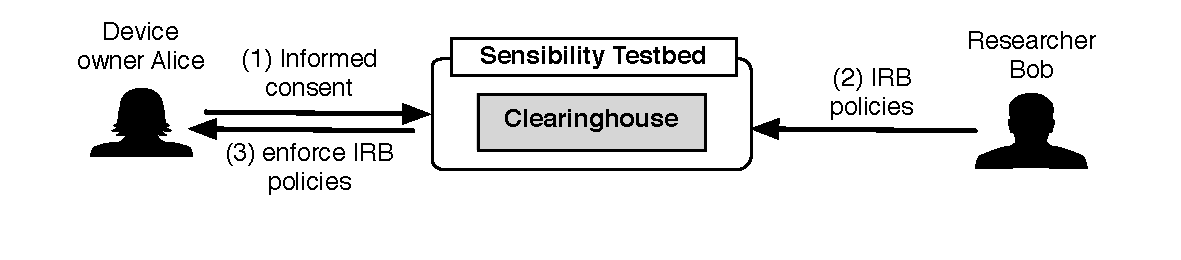
\includegraphics[width=\columnwidth]{figs/irb.pdf}}
%\vspace*{-20pt}
\caption{\small A high-level walkthrough. \label{fig-walkthrough}}
\end{figure}

The basic operation of \sysname involves four separate 
parties: a \textit{device owner} interested in participating in 
experiments, a \textit{clearinghouse} that discovers the
participating devices, and configures privacy policies on the 
devices,  a \textit{researcher} seeking to run experiments on 
remote devices. 
In the following, we assume that Alice, a device owner, participates in 
the testbed, while a researcher, Bob, wants to runs code on \sysname 
using Alice's device, among other devices.

For Bob, the steps required to run an experiment include
%on \sysname roughly fall into two categories: 
IRB approval for his experiment, and code deployment.
Bob first %designs his experiment, and 
%possibly tests its feasibility on his own device (on which he can 
%use the same \sysname app but does not need IRB approval to access it). 
%Following this, he 
registers his experiment on the \sysname clearinghouse, where he 
specifies the sensors and sensor accuracy that his experiment 
requires through a web form. Suppose that the goal of Bob's experiment is to determine the cellular service
quality in major cities. His experiment therefore needs to obtain location information
of individual devices, their cellular service provider, network
type (3G, 4G, LTE, etc.), and signal strength. 
The clearinghouse's form provides Bob 
%summarizing the request. 
with a list of available sensors and their possible privacy configurations. 
Bob then requests approval for his experiment from his 
institution's IRB, supplying his experiment description using the clearinghouse form, the \sysname's approved 
IRB, and any additional information about the testbed as needed by his institution. 
The process how Bob specifies IRB policies is described in details in 
Section~\ref{sec-ch}. Once Bob's IRB approves the experiment, he 
uploads the confirmation to \sysname's clearinghouse, and is finally 
granted the permission to access devices to deploy his experiment 
and collect data, as will be described in Section~\ref{sec-emt}.

In order for Alice to participate in Sensibility Testbed,
she starts by installing the Sensibility Testbed app from 
the Android app store~\cite{sensibility-app}. After downloading the app, 
Alice is informed about the testbed's privacy and usage policy 
in a consent form and must give consent before participating.
She can opt out of the testbed by uninstalling the app, opt out of
an individual experiment, and set local sensor policies that
will supersede Bob's IRB policies (Section~\ref{sec-repy}). This
protocol for research with mobile device sensors has been approved by
the IRB at New York University (IRB \# 15-10751).  

\begin{comment}
Bob completes a series of steps to deploy his experiment on \sysname.
He first fills out a form at a \sysname website 
(Section~\ref{sec-ch}), which has a list of checkboxes for device sensors 
and text boxes indicating the precision and frequency that Bob can access 
each sensor. These boxes provide the default policies of \sysname, and 
Bob can only indicate data of coarser granularity. \jill{i thought this process was automated?}
Bob then downloads 
documents to provide to his IRB that 
explains the details about his experiment, \sysname and the technical 
restrictions his experiment will have. Bob then obtains IRB approval at 
his institution, provides his institution's IRB policies to the 
\sysname website, and signs up for his experiment. 

The form that Bob filled out on the \sysname website is used to
enforce a set of technical restrictions for his experiment.  This means
that even if Bob makes an error in his code or his code is malicious, his 
experiment is still restricted in the data it can acquire. 
\yanyan{how can restricting data prevent errors?} Therefore, Bob's IRB 
policies which request access to cellular signal strength and network type, would result 
in his experiment being blocked from reading the cellular roaming status and cell 
IDs. Note that the latter information is accessible with the same 
Android permission, but is blocked by \sysname.  This
protocol for research with mobile device sensors has been approved by
the IRB at New York University (IRB \# 15-10751).  

Note that the policies set limits to the precision of data that Bob can request
for many sensors (e.g., preventing access to the raw MAC address of the device).
If Bob has a legitimate need for this data and can appropriately secure it,
Bob can request such access by also passing his locally approved request 
through \sysname's IRB.  This additional check ensures not only that Bob's 
handling and access to the data is appropriate, but ensures that this does
not violate Alice's privacy and usage policy with the Sensibility Testbed.
%When Bob's IRB wants to access information that is more sensitive than
%what is described in NYU IRB, \yanyan{Justin, help!}  

Once Bob's experiment has been approved and the appropriate privacy
restrictions are identified, Bob can obtain remote devices, and run his experiment on the
devices of participants like Alice (Section~\ref{sec-emt}). On Alice's device, the app displays a 
list of running experiments and their policies. If Alice does not agree with
sharing her MAC address, she can opt out of Bob's experiment. 
%\cappos{how is this updated?  Does Alice see this before or after an 
%experiment may run?  How much "lead time" does Alice get to opt-out
%before the experiment happens?}
%\cappos{Do you want to say something about informed consent here or
%does it fit better later?} 
Alice's informed consent to Sensibility Testbed
ensures that Bob does not need to individually recruit Alice to include
her device in his study.

This work flow is shown in Figure~\ref{fig-walkthrough}. \jill{let's add how Bob gets the 
data from Alice's device in Figure 1} \sysname
acts as an intermediate between the device owner and researcher, 
where the device owners give their informed consent, and researchers
provide their IRB policies. The researchers do not recruit
device owners directly for each experiment, and the testbed infrastructure 
enforces the IRB policies on behalf of the researcher. 

\sysname's default policies are described next.
\end{comment}

%Device owners like Alice participate in Sensibility Testbed by p.

%These policies restrict what and how data can be accessed by the 
%researcher. 
%into data blurring layers that are enforced on
%mobile devices. Such a process can protect device
%owners' personal information. 
%Researchers' code runs in a sandbox that isolates the code from the 
%rest of the device host system. 
%To control the execution of code, Bob uses his own 
%desktop or laptop computer to manage the 
%experiments via the experiment manager. It deploys 
%and runs experiments in sandboxes on remote devices that are 
%acquired through the clearinghouse.

%\textbf{Usage scenario 1: Smartphone owner volunteers as a testbed participant.}
%Alice downloads the Sensibility Testbed app from the Google Play 
%Store~\cite{sensibility-app}, which will install Repy and other software on her phone.
%The app displays a consent form, \yanyan{cite link} containing the testbed's 
%general usage policy. Alice must review and must agree to this 
%policy before installation. If Alice gives her consent, her device will be 
%installed with the Repy sandbox, the native Android code to 
%start or stop the sandbox, and an interface to communicate with the testbed 
%infrastructure (particularly the clearinghouse, described below). 
%By agreeing to our general usage policy, any device 
%owner, regardless of age, country, or background, need only to opt into our testbed as a
%volunteer \textit{once}, at the time of app installation. 
%%As a result, an 
%%researcher like Bob who wants to conduct an experiment 
%%%requests devices through our clearinghouse, which assigns 
%%%them devices from a set of available resources. As a result, 
%%%the researcher
%%does not need to get consent from each subject for each individual
%%experiment. \lois{is the previous sentence needed? I don't think so} 
%The testbed thus greatly simplifies the process for both the 
%device owners and experimenters. 


\begin{table*}
\scriptsize
\centering

\bgroup
\def\arraystretch{1.15}% % for table padding
\begin{tabular}{|p{3cm}|p{8cm}|p{4cm}|}
\hline
{\bf Goals\textsuperscript{*}}  & {\bf Sensor data} & {\bf Default policy\textsuperscript{\dag}}  
\\ \hline \hline

\multirow{8}{3cm}{Support research projects. \yanyan{this is not a prevention goal tho.}} 
& Battery status (charging/discharging), temperature, 
 technology, health (good/overheat), battery level, voltage, plug-in type. & 
 \multirow{8}{4cm}{Full precision, round-up (if numeric), or constant.} \\ \cline{2-2}
 
& Bluetooth scan mode, state (enabled/disabled). &  \\ \cline{2-2}
 
& Cellular network roaming status, SIM card status (ready/absent), 
phone status (idle/busy), signal strength. &   \\ \cline{2-2}

& Location service provider. & \\ \cline{2-2}

& WiFi link speed, association state, nearby routers' frequency, signal strength. & \\ \cline{2-2}
  
& Vibrate mode, screen settings (on/off, brightness, timeout), media/ringer 
volume. &  \\ \hline 

%%%%%%%%%%%%%%%%%%%%%%%%%%%%%%%%%%%%%%

\multirow{2}{*}{Prevent keyloggers.} & Motion sensors: accelerometer, gyroscope, magnetometer, 
orientation, ambient light. & Full precision, round-up, random rotation, constant; restrict 
 access frequency. \\ \hline 

%%%%%%%%%%%%%%%%%%%%%%%%%%%%%%%%%%%%%%

\multirow{12}{*}{Prevent locating a device.} & 
\multirow{3}{*}{Latitude, longitude, altitude.}  & Approximate to the nearest 
zipcode region, or city/state/country center; restrict access frequency.  \\\cline{2-3}
%& & Speed. & Round-up, or constant. & \\\cline{3-4}

& \multirow{2}{*}{Nearby Bluetooth device names.} & Hashed device names; restrict 
 access frequency.  \\ \cline{2-3}

& \multirow{2}{*}{Cellular network cell ID, neighboring cell ID(s).} & Randomized ID; restrict access 
frequency.   \\ \cline{2-3}

& \multirow{2}{*}{Cellular network operator ID and name, country code, area code.} & Hashed ID, names, 
and code; restrict access frequency.  \\ \cline{2-3}

& WiFi connection information (SSID and MAC address of the currently connected router). 
& \multirow{3}{4.1cm}{Hashed SSID, randomized MAC address; restrict 
 access frequency.} \\ \cline{2-2}  
& WiFi scan result (nearby WiFi routers' SSIDs and MAC addresses) & \\ \hline 

%%%%%%%%%%%%%%%%%%%%%%%%%%%%%%%%%%%%%%

\multirow{5}{3cm}{Prevent identifying a device owner.} & \multirow{2}{*}{Bluetooth MAC 
address, local name.}  & Randomized MAC address, hashed device names. \\ \cline{2-3}

& Cellular device ID, incoming number.  & Randomized ID and number. \\ \cline{2-3}

& \multirow{2}{*}{WiFi connection information (device MAC address, IP address).} & 
Randomized MAC address, hashed IP address.  \\ \hline 

%%%%%%%%%%%%%%%%%%%%%%%%%%%%%%%%%%%%%%
%Start/stop activities & & & \xmark \\ \hline 
%Running applications & & & \xmark \\ \hline 
\multirow{2}{*}{Prevent video/ audio recording.} & 
Take pictures, record videosn using a camera. & \multirow{5}{*}{Disabled} \\ \cline{2-2} 

& Voice record using a microphone. & \\ \cline{1-2} 

\multirow{2}{*}{Prevent actions for owner.}& Scan barcode, search, etc., using an Intent.  &  \\ \cline{2-2} 

& Send/receive messages, delete messages, dial/pick up phone calls. & \\  \cline{1-2} 

Protect owner's contacts. & Contact list of the device owner in an address book. & \\ \hline 

\multicolumn{3}{l}{\textsuperscript{*}\scriptsize These goals are the common goals, though uncommon 
goals exist. For example, motion sensors can be used to fingerprint devices~\cite{bojinov2014mobile}, 
or record conversations~\cite{michalevsky2014gyrophone}.} \\ 

\multicolumn{3}{l}{\textsuperscript{\dag}\scriptsize As new threats emerge, we plan to adjust the default
policies.} \\ 

\end{tabular}
\egroup

\caption{\small Sensibility Testbed's default policies for sensor data.}
\label{tab:default}
%\vspace{-10pt}
\end{table*}

\subsection{Default Policies}\label{sec-policy-design}

Policies govern at which accuracy and rate a sandboxed experiment can 
access sensors on a device, if any. 
The goal of \sysname is to protect the device owner's privacy, while making
the data from mobile devices useful for a wide range of research. 
%As mentioned earlier, failure to recognize the vulnerability of
%certain sensors was a key reason for privacy breaches. 
Sensibility Testbed uses \textit{default policies} to specify how 
different types of sensors can be accessed to prevent common privacy and
security attacks, %To privide such protection, \sysname 
%classifies sensors as 
%of low, moderate, or high risk. Sensors of high risk are not accessable to 
%researchers by default, and the sensors of low and moderate risk are further 
%protected by the default policies.
%uses a set of policies to prevent a range of attacks, 
as listed in Table~\ref{tab:default}. 
%These policies roughly fall into three categories.
Researchers can further customize the policies through their IRB
to access sensors at a coarser data granularity. The default and 
customized policies would then be automatically enforced by the \sysname 
infrastructure. 
%\cappos{Shouldn't this detail come earlier?  Why is this here instead?}
Also, the device owner may add their own policies which have ultimate 
control over the maximum sensor access accuracy and rate that an 
experiment can attain.

%\textbf{Category 1.}
The \textit{default policies} disable highly sensitive sensors 
such as cameras and microphones. 
If a microphone is controlled by a malicious party, for example, it can be used to 
intelligently choose data of a higher value to record, such as a credit card 
number or password~\cite{zhang2015leave}. Cameras face similar
risks. Additionally, the default policies disable interrupting actions, such as 
making phone calls, scanning a barcode on behalf of the device owner, 
and accessing an address book. 

%\textbf{Category 2.}
Given our analysis of privacy attacks in the current literature, 
we have identified the three 
most common 
risks for device owners (Section~\ref{sec-our-policies}): (1) identifying a device or its owner, 
(2) locating a device, and (3) inferring keys strokes typed by a device owner. 
As shown in Table~\ref{tab:default}, 
sensor data like MAC address and device ID can be used to identify a device, while latitude, longitude, cell 
IDs, and a WiFi router's SSID can be use to locate a 
device. Motion sensors like accelerometer and gyroscope can also be used
as keyloggers to infer keys typed or icons tapped on a 
smartphone. Compared to cameras and microphones, these 
sensors normally require a background process that continuously 
collects the data, or a sophisticated algorithm that constantly learns 
about the patterns of data generated. 
Therefore, Sensibility Testbed's default policies 
blur data from these sensors, but don't disable them completely. 
For example, the default policies enforce randomized MAC addresses in a 
Bluetooth and WiFi network, approximated location coordinates, and 
control the frequency of access to motion sensor data. Note that keyloggers (risk 3)
are more effective when the access frequency to motion sensors is 
high: Previous work such as ACCessory~\cite{owusu2012accessory}, 
TapPrints~\cite{miluzzo2012tapprints}, TapLogger~\cite{xu2012taplogger}, 
and other projects~\cite{aviv2012practicality} showed that when the 
frequency to get motion sensor data is above a certain threshold, the keyloggers' 
learning algorithms become much more accurate.  
Using \sysname's default policies, we can limit 
motion sensors to be accessed at a rate lower than this threshold. 


%\textbf{Category 3.}
%\sysname's default policies allow research 
%projects to get data at a level that is meaningful. For example, 
%projects that are interested in monitoring human activity, wireless network 
%performance, etc., sensor values are allowed at the granularity that is safe 
%according to the researcher's IRB. 

%The default policies currently allow this data to be 
%accessed with full precision (accuracy can be reduced if the IRB
%does not require full precision), since data such as cellular signal strength and WiFi 
%link speed is typically only meaningful with highest accuracy. While it is true that
%certain data like battery information can be used to infer the location of 
%a device, such techniques only works in conjunction with other data 
%such as cellular data usage~\cite{michalevsky2015powerspy}\footnote{\scriptsize 
%The tracking works by measuring the overall power consumption 
%by the phone's cellular radio. Cellular radio power consumption depends 
%on the distance to the nearest cellular tower and any obstacles between 
%the phone and tower. This combination of factors creates a unique power 
%consumption profile for each geographic location~\cite{battery-use}.}. 
%Since the latter data has been protected by aforementioned policies, such 
%complex privacy attacks become less effective. \jill{not sure if this argument is strong
%because we can't account for every possible combination}

\begin{comment}
\textbf{Risk categorization.}
%Even if an IRB happened 
%to approve such a policy, there are certain sensors that the testbed's
%own IRB designates as off-limits due to the high risk associated with 
%potential breaches. 
%and for which access can be pre-approved with the
%researcher's local IRB. 
%Only those sensors listed on our project 
%wiki page~\cite{sensor-api} are accessible to a researcher. 
A summary of these sensors is listed in Table~\ref{tab:default}.
%with each one categorized as . 
%The list of sensors that Sensibility Testbed provides are all of moderate 
%to low privacy risks (marked by \tickmark), and the testbed further provides policy enforcement
%(Section~\ref{sec-policy}) to protect all the sensor data. Sensors 
%such as cameras and microphones that are deemed sensitive are not 
%exposed to experiment code by default (marked by \xmark). 
The classification into low, moderate or high 
privacy risk is motivated by the Android system, where 
permissions are categorized into different protection levels~\cite{level}:
\textit{normal} permissions are automatically granted to the apps, 
\textit{dangerous} permissions are given based upon the 
user's consent, and so on. In our case, 
%we divide sensors into different risk levels, as shown 
%in Table~\ref{tab:default}. 
%Sensors with low to moderate risk are 
%allowed and protected by IRB policies. Sensors of high risk are 
%disabled by default. 
we divide sensors into different risk levels by the consequences and 
difficulties of a potential attack. If a microphone is controlled by 
a malicious party, it can be used to intelligently choose data of a 
higher value (e.g., credit card number, password) to record~\cite{zhang2015leave}. On the other 
hand, in order to infer a credit card number or password typed on a 
smartphone using motion sensors, the attack requires the installation of 
a sophisticated algorithm on the device that constantly learns about  
the patterns of data generated by accelerometer or gyroscope. In contrast,
using battery information alone is not sufficient to create a fingerprint 
for each device. Different information and mutiple occurrences need to
be pieced together to extract this data~\cite{battery-priv}. Therefore, 
compared to motion sensors, a microphone is considered a higher risk, 
and a battery is a significantly lower risk.

\textbf{Default and customizable policies.}
For sensors of low and moderate risk, the default policies are listed in 
Table~\ref{tab:default}. Our principle to design the the default policies 
is that a device or its owner cannot be identifiable, but research projects
are allowed to get data at a level that is meaningful. For example, Bluetooth
and WiFi network MAC addresses can uniquely identify a device, therefore, 
the default policy for these sensor data is to return randomized MAC 
addresses to an experiment, as in~\cite{aditya2014encore}, and this is 
mandatory (marked by N/A). For research projects that are interested 
in monitoring human activity, wireless network performance, etc., sensor
values are allowed to the granularity that is safe. Some data can be 
accessed at full precision (cellular signal strength, WiFi link speed), 
whereas others have an upper bound on their access frequency. 
\yanyan{how to add frequency to the table?}

\end{comment}


As a consequence of our analysis of previous work, \sysname blurs (or 
even disables access to) sensor data by default.
However, if a finer-grained access is critical to the study, access 
must be requested by going through the \sysname's IRB, in addition to the 
researcher's IRB. Even if both IRBs consent that access at elevated accuracy 
should be granted, the local policies configured by the device owner still 
supersede both \sysname's default policies and the researcher's IRB policies, 
and may still block fine-grained access. We further describe this hierarchy 
of policies in Section~\ref{sec-repy}.

\sysname's default policies are set to appropriate levels to protect against 
known attacks today. %as shown in our analysis in Section~\ref{sec-our-policies}. 
However, these levels will need to change over time as
new attacks emerge and become available. \sysname's IRB allows adjusting 
of sensor access restrictions, therefore making the default policies
stronger over time as they adjust to new attacks. It is also important to note that 
if a researcher's IRB allows access to non-sensitive sensor data, \sysname will 
enable the researcher to obtain that data without control over what the data is used for.
A researcher may succeed in finding a new attack by combining this data with other 
information, for example. However, given the 
knowledge of the new attack, \sysname can update its default policies to prevent against
this type of attack happening with future use. 
%\yanyan{Justin, help!} 
%\cappos{Don't you have some things you would never allow even if the NYU IRB
%approves it?}
%\lois{following up on Yanyan's comment--If the Testbed's IRB says this expanded access is permissable, are the device owner's notified and can they opt out of this study? Otherwise, that would be a direct violation of the privacy protection you claim to give them}
%\lois{I did not touch these last two paragraphs because I still don't know about  the opt-out policy for individuals if this permission is given}
%Depending on the experiment description provided by the 
%researcher, the fields marked with a (*) are the ones that will be blurred.
%
%
%
%As a result, Sensibility Testbed does not
%provide unfettered access to all sensors. 
%Access to sensors of
%higher risk, e.g., the policies that request restricted sensor data, 
%or at higher frequencies than our default policies, 
%needs to go through the Sensibility Testbed's IRB,
%in addition to the researcher's IRB. 
%In most cases, we expect
%that researchers need only go through their local IRB to get
%the sensor access they need for their experiment. 


